\chapter{What is a Display Server?}
\label{ch:what-is-display-server}

\epigraph{Every pixel you see on your screen is the result of a complex dance between hardware, kernel, and userspace software. The display server is the choreographer.}{--- Anonymous}

\section{Introduction: The Invisible Infrastructure}

Every time you move your mouse cursor across the screen, click a button, type in a text editor, or watch a video, you're interacting with one of the most fundamental yet invisible components of your computer system: the \textbf{display server}.

Most computer users have never heard of a display server, yet it's working continuously, orchestrating every visual element you see. Understanding what a display server is—and why it matters—is the foundation for understanding Wayland.

\begin{importantbox}
A display server is the intermediary between your applications and your display hardware. It's responsible for drawing windows, handling input, and coordinating which applications get to show what on your screen.
\end{importantbox}

\section{The Fundamental Problem}

\subsection{Why Do We Need a Display Server?}

Imagine a world without a display server. What would happen?

\paragraph{The Chaos of Direct Hardware Access}

Consider a simple scenario: you have two programs running—a web browser and a text editor. Both want to display content on your screen. Without a display server:

\begin{enumerate}[leftmargin=*]
    \item Both programs would need to directly control the graphics hardware
    \item They would fight over which pixels belong to whom
    \item There would be no concept of "windows"—just a single framebuffer
    \item One program could overwrite another's pixels
    \item Input events (keyboard, mouse) would have no clear destination
    \item No program could know where on the screen it should draw
\end{enumerate}

This is not hypothetical. This is exactly how early computers worked, and it's still how some embedded systems operate today. Each application had complete control of the screen, and only one application could run at a time (at least visibly).

\begin{examplebox}
\textbf{Real-World Analogy: The Whiteboard}

Imagine a shared whiteboard in an office with no rules:
\begin{itemize}
    \item Anyone can write anywhere at any time
    \item People write over each other's content
    \item There's no organization or boundaries
    \item No one knows whose turn it is to use the board
\end{itemize}

A display server is like establishing rules: each person gets a designated area, takes turns, and a coordinator ensures everyone's content is visible and properly organized.
\end{examplebox}

\subsection{The Core Responsibilities}

A display server solves this chaos by providing several critical services:

\paragraph{1. Window Management Coordination}

The display server doesn't necessarily manage windows itself (we'll get to this distinction later), but it provides the infrastructure for windows to exist. It:

\begin{itemize}[leftmargin=*]
    \item Allocates screen regions to different applications
    \item Maintains the window hierarchy (which window is on top)
    \item Handles window overlap and composition
    \item Provides APIs for creating and manipulating windows
\end{itemize}

\paragraph{2. Input Event Routing}

When you press a key or move your mouse:

\begin{itemize}[leftmargin=*]
    \item The hardware generates an event
    \item The kernel captures this event
    \item The display server determines which application should receive it
    \item The event is delivered to the appropriate application
\end{itemize}

Without a display server, which application should get the keystroke? The answer would be ambiguous.

\paragraph{3. Graphics Arbitration}

Modern graphics hardware is complex and powerful, but it's also a shared resource. The display server:

\begin{itemize}[leftmargin=*]
    \item Manages access to the GPU
    \item Coordinates rendering operations
    \item Handles buffer management
    \item Ensures smooth visual output
\end{itemize}

\paragraph{4. Display Output Management}

The display server manages:

\begin{itemize}[leftmargin=*]
    \item Multiple monitors
    \item Display resolution and refresh rate
    \item Display rotation and scaling
    \item Hot-plugging of displays
\end{itemize}

\section{The Abstraction Layer Model}

To understand where the display server fits in the system, let's examine the complete stack:

\begin{figure}[htbp]
\centering
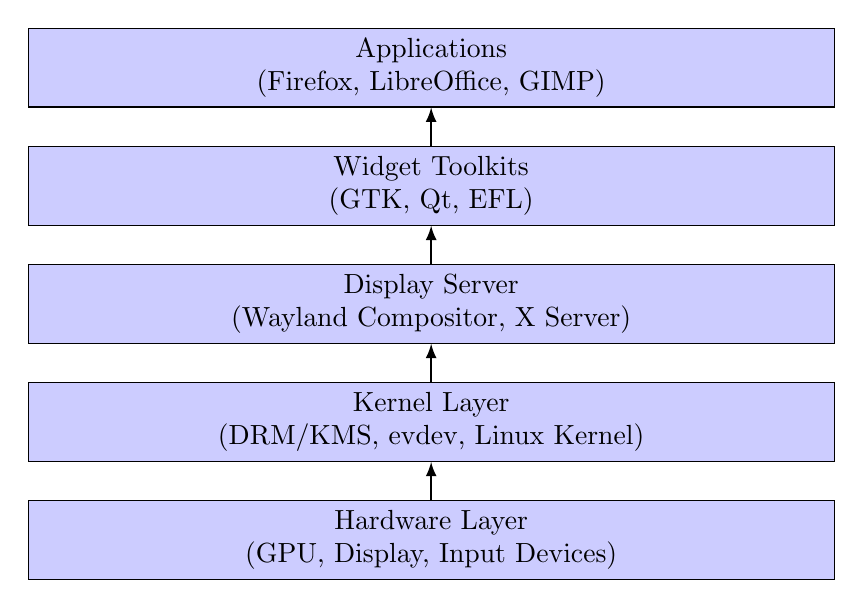
\begin{tikzpicture}[
    box/.style={rectangle, draw, fill=blue!20, text width=10cm, align=center, minimum height=1cm},
    arrow/.style={->, >=latex, thick}
]
    \node[box] (hardware) at (0,0) {Hardware Layer\\(GPU, Display, Input Devices)};
    \node[box] (kernel) at (0,1.5) {Kernel Layer\\(DRM/KMS, evdev, Linux Kernel)};
    \node[box] (display) at (0,3) {Display Server\\(Wayland Compositor, X Server)};
    \node[box] (toolkit) at (0,4.5) {Widget Toolkits\\(GTK, Qt, EFL)};
    \node[box] (apps) at (0,6) {Applications\\(Firefox, LibreOffice, GIMP)};

    \draw[arrow] (hardware) -- (kernel);
    \draw[arrow] (kernel) -- (display);
    \draw[arrow] (display) -- (toolkit);
    \draw[arrow] (toolkit) -- (apps);
\end{tikzpicture}
\caption{The display system stack from hardware to applications}
\label{fig:display-stack}
\end{figure}

Let's examine each layer:

\subsection{Hardware Layer}

At the bottom, we have the physical components:

\begin{itemize}[leftmargin=*]
    \item \textbf{GPU (Graphics Processing Unit)}: Renders graphics, performs computations
    \item \textbf{Display Controller}: Converts framebuffers to video signals
    \item \textbf{Physical Displays}: Monitors, laptop screens
    \item \textbf{Input Devices}: Keyboards, mice, touchpads, touchscreens
\end{itemize}

These components speak the language of electricity, signals, and hardware protocols.

\subsection{Kernel Layer}

The Linux kernel provides device drivers and interfaces:

\begin{itemize}[leftmargin=*]
    \item \textbf{DRM (Direct Rendering Manager)}: GPU driver interface
    \item \textbf{KMS (Kernel Mode Setting)}: Display mode setting
    \item \textbf{evdev}: Input event device interface
    \item \textbf{Input subsystem}: Processes raw input events
\end{itemize}

The kernel translates hardware operations into software-accessible interfaces, but it doesn't make policy decisions about which application gets what resources.

\begin{notebox}
\textbf{Why doesn't the kernel handle display serving?}

The Linux kernel follows the principle of \textit{mechanism, not policy}. The kernel provides the mechanisms (interfaces to hardware), but policy decisions (which window is on top, where to route input) belong in userspace where they can be flexible and changeable without kernel modifications.
\end{notebox}

\subsection{Display Server Layer}

This is where our focus lies. The display server:

\begin{itemize}[leftmargin=*]
    \item Receives output from applications
    \item Receives input from the kernel
    \item Arbitrates between competing applications
    \item Manages the visual presentation
    \item Routes input to the correct application
\end{itemize}

\subsection{Toolkit Layer}

Widget toolkits (GTK, Qt, etc.) provide higher-level abstractions:

\begin{itemize}[leftmargin=*]
    \item Buttons, menus, text boxes
    \item Theme and styling
    \item Layout management
    \item Event handling
\end{itemize}

These toolkits \textit{use} the display server but don't replace it.

\subsection{Application Layer}

Finally, the applications themselves—the programs users actually run.

\section{Two Architectural Approaches}

Historically, there have been two main architectural approaches to display servers:

\subsection{The Traditional Model: Centralized Display Server}

In this model, exemplified by \xorg{}, the display server is a central, powerful component that:

\begin{itemize}[leftmargin=*]
    \item Maintains all window state
    \item Performs all rendering
    \item Handles all input
    \item Manages all displays
    \item Contains font rendering, drawing primitives, etc.
\end{itemize}

\begin{figure}[htbp]
\centering
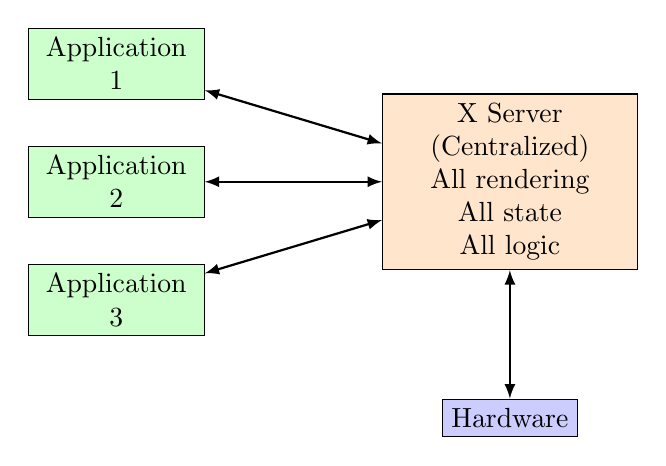
\begin{tikzpicture}[
    client/.style={rectangle, draw, fill=green!20, text width=2cm, align=center, minimum height=0.8cm},
    server/.style={rectangle, draw, fill=orange!20, text width=3cm, align=center, minimum height=2cm},
    arrow/.style={<->, >=latex, thick}
]
    \node[client] (app1) at (0,3) {Application 1};
    \node[client] (app2) at (0,1.5) {Application 2};
    \node[client] (app3) at (0,0) {Application 3};

    \node[server] (xserver) at (5,1.5) {X Server\\(Centralized)\\All rendering\\All state\\All logic};

    \draw[arrow] (app1) -- (xserver);
    \draw[arrow] (app2) -- (xserver);
    \draw[arrow] (app3) -- (xserver);

    \node[draw, fill=blue!20] (hw) at (5,-1.5) {Hardware};
    \draw[arrow] (xserver) -- (hw);
\end{tikzpicture}
\caption{Traditional centralized display server model (\xorg{})}
\label{fig:x11-model}
\end{figure}

\paragraph{Advantages:}
\begin{itemize}[leftmargin=*]
    \item Consistent behavior across applications
    \item Thin clients possible (applications can be very simple)
    \item Network transparency (can run applications remotely)
\end{itemize}

\paragraph{Disadvantages:}
\begin{itemize}[leftmargin=*]
    \item Complex, monolithic server
    \item Performance bottleneck
    \item Security concerns (all applications can see all windows)
    \item Difficult to modernize
\end{itemize}

\subsection{The Modern Model: Compositor-Based}

The Wayland approach is fundamentally different:

\begin{itemize}[leftmargin=*]
    \item Applications render their own windows
    \item The compositor combines (composes) these windows
    \item Each client is isolated from others
    \item Much of the logic moves to clients and toolkits
\end{itemize}

\begin{figure}[htbp]
\centering
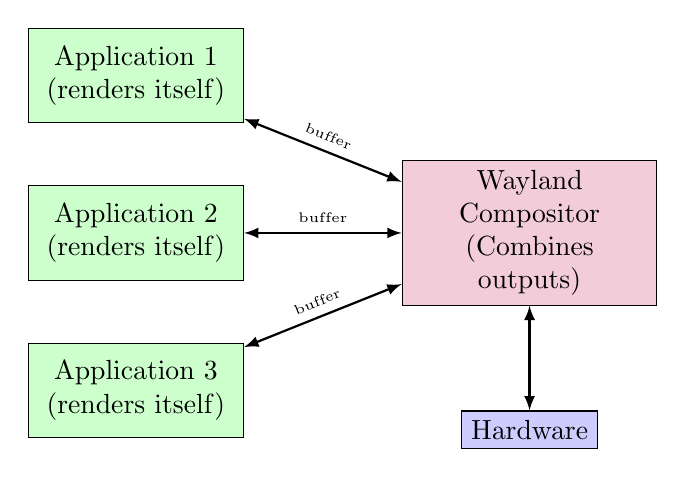
\begin{tikzpicture}[
    client/.style={rectangle, draw, fill=green!20, text width=2.5cm, align=center, minimum height=1.2cm},
    compositor/.style={rectangle, draw, fill=purple!20, text width=3cm, align=center, minimum height=1.5cm},
    arrow/.style={<->, >=latex, thick}
]
    \node[client] (app1) at (0,3) {Application 1\\(renders itself)};
    \node[client] (app2) at (0,1) {Application 2\\(renders itself)};
    \node[client] (app3) at (0,-1) {Application 3\\(renders itself)};

    \node[compositor] (comp) at (5,1) {Wayland\\Compositor\\(Combines\\outputs)};

    \draw[arrow] (app1) -- (comp) node[midway, above, sloped, font=\tiny] {buffer};
    \draw[arrow] (app2) -- (comp) node[midway, above, sloped, font=\tiny] {buffer};
    \draw[arrow] (app3) -- (comp) node[midway, above, sloped, font=\tiny] {buffer};

    \node[draw, fill=blue!20] (hw) at (5,-1.5) {Hardware};
    \draw[arrow] (comp) -- (hw);
\end{tikzpicture}
\caption{Modern compositor-based model (Wayland)}
\label{fig:wayland-model}
\end{figure}

\paragraph{Advantages:}
\begin{itemize}[leftmargin=*]
    \item Better performance (less copying of data)
    \item Improved security (application isolation)
    \item Simpler core protocol
    \item Flexibility for compositors to innovate
\end{itemize}

\paragraph{Disadvantages:}
\begin{itemize}[leftmargin=*]
    \item More complexity in toolkits
    \item No built-in network transparency
    \item Requires more from applications
\end{itemize}

\begin{designbox}
\textbf{Why the shift from centralized to distributed?}

The move from X11's centralized model to Wayland's distributed model reflects several modern realities:

\begin{enumerate}
    \item \textbf{Hardware has changed}: Modern GPUs are extremely powerful, and having applications render directly is efficient.
    \item \textbf{Security matters more}: Application isolation is now a priority.
    \item \textbf{Network transparency isn't free}: The cost of building it into the core protocol affects local performance.
    \item \textbf{Composition is universal}: Every modern desktop uses composition effects; they should be first-class.
\end{enumerate}
\end{designbox}

\section{Key Concepts and Terminology}

Before we proceed deeper, let's establish some fundamental terminology:

\subsection{Client vs. Server}

\begin{definition}[Client]
A \textbf{client} is an application that wants to display graphical output. Examples: web browser, text editor, video player.
\end{definition}

\begin{definition}[Server]
The \textbf{server} (or compositor in Wayland terminology) is the system component that manages the display and coordinates clients.
\end{definition}

\begin{warningbox}
The terms "client" and "server" can be confusing because they're opposite to what many people expect. The application you run (Firefox, for example) is the \textit{client}, while the system service (Wayland compositor) is the \textit{server}.

Think of it this way: the applications are clients that \textit{request services} from the display server.
\end{warningbox}

\subsection{Window vs. Surface}

\begin{definition}[Window]
In traditional terminology, a \textbf{window} is a rectangular area on screen containing application content with decorations (title bar, borders, etc.).
\end{definition}

\begin{definition}[Surface]
A \textbf{surface} is a more fundamental concept: it's a rectangular buffer of pixels that can be displayed. A window might consist of multiple surfaces.
\end{definition}

Wayland uses the term "surface" more often than "window" because it's more precise and general.

\subsection{Compositor}

\begin{definition}[Compositor]
A \textbf{compositor} is a component that combines multiple graphical elements (surfaces) into a single final image for display.
\end{definition}

In Wayland, the compositor \textit{is} the display server. This is a key distinction from X11, where composition was added later as an extension.

\subsection{Buffer}

\begin{definition}[Buffer]
A \textbf{buffer} is a region of memory containing pixel data. Clients render into buffers and send them to the compositor for display.
\end{definition}

\subsection{Protocol}

\begin{definition}[Protocol]
A \textbf{protocol} is the formal specification of how clients and servers communicate. It defines the messages they can exchange and the rules for their interaction.
\end{definition}

\section{What a Display Server Is NOT}

It's equally important to understand what a display server is \textit{not}:

\subsection{Not a Window Manager}

A \textbf{window manager} decides:
\begin{itemize}[leftmargin=*]
    \item Window placement on screen
    \item Window decorations (title bars, borders)
    \item Window behavior (minimize, maximize, close)
    \item Keyboard shortcuts for window operations
\end{itemize}

In X11, the window manager and display server are separate. In Wayland, these roles are typically combined in the compositor, but conceptually they're still distinct functions.

\subsection{Not a Desktop Environment}

A \textbf{desktop environment} provides:
\begin{itemize}[leftmargin=*]
    \item Panels and taskbars
    \item Application launchers
    \item System settings
    \item File managers
    \item Themes and appearance
\end{itemize}

The display server is a much lower-level component that the desktop environment builds upon.

\subsection{Not the Graphics Driver}

Graphics drivers live in the kernel and communicate directly with hardware. The display server uses drivers but is not itself a driver.

\subsection{Not a Rendering Engine}

While the display server handles composition, applications (and their toolkits) do most of their own rendering. The display server doesn't typically draw buttons, text, or application-specific graphics.

\section{The Display Server in Context}

\subsection{Historical Context}

Display servers emerged because:

\begin{enumerate}[leftmargin=*]
    \item Early computers could only run one program at a time
    \item Time-sharing systems needed to share displays among multiple users
    \item Graphical interfaces needed coordination between multiple programs
    \item Network computing required remote display capability
\end{enumerate}

\subsection{Modern Requirements}

Today's display servers must handle:

\begin{itemize}[leftmargin=*]
    \item High-resolution displays (4K, 5K, 8K)
    \item High refresh rates (120Hz, 144Hz, 240Hz)
    \item Multiple monitors with different properties
    \item Touch input and gestures
    \item Hardware acceleration for video and 3D graphics
    \item Accessibility features
    \item Security isolation between applications
    \item Power efficiency for mobile devices
\end{itemize}

\section{Why This Matters}

Understanding what a display server is and why it exists is crucial for several reasons:

\subsection{For Users}

Even if you never program a display server, understanding this layer helps you:

\begin{itemize}[leftmargin=*]
    \item Troubleshoot display issues
    \item Understand performance characteristics
    \item Make informed choices about desktop environments
    \item Appreciate the complexity behind the simple act of moving windows
\end{itemize}

\subsection{For Developers}

If you're developing graphical applications:

\begin{itemize}[leftmargin=*]
    \item You'll interact with the display server through toolkits
    \item Understanding the underlying model helps you make better design decisions
    \item Performance optimization requires understanding the full stack
    \item Porting between X11 and Wayland requires understanding both models
\end{itemize}

\subsection{For System Architects}

Understanding display servers is essential for:

\begin{itemize}[leftmargin=*]
    \item Designing efficient graphical systems
    \item Implementing security policies
    \item Optimizing resource usage
    \item Creating embedded or specialized systems
\end{itemize}

\section{Summary}

In this chapter, we've established that:

\begin{enumerate}[leftmargin=*]
    \item A display server is the intermediary between applications and display hardware
    \item It solves the fundamental problem of multiple applications sharing visual and input resources
    \item It sits between the kernel and applications in the system stack
    \item There are two main architectural models: centralized (X11) and compositor-based (Wayland)
    \item The display server is distinct from window managers, desktop environments, and drivers
    \item Modern display servers face complex requirements around performance, security, and diverse hardware
\end{enumerate}

\begin{notebox}
\textbf{Key Takeaway}

A display server is essential infrastructure that you interact with constantly but rarely think about. It's the invisible choreographer that makes graphical computing possible, coordinating the complex dance between your applications, input devices, and display hardware.
\end{notebox}

In the next chapter, we'll explore the history of X11—the dominant display server for over 30 years—to understand both its achievements and the limitations that led to Wayland's creation.

\section{Further Reading}

\begin{itemize}[leftmargin=*]
    \item The X Window System architecture documentation
    \item "The Linux Graphics Stack" by Martin Peres
    \item Kernel documentation on DRM/KMS
    \item Historical papers on windowing systems from the 1980s
\end{itemize}
